
\section{Lichtschranken-Station}
Hier wird die grundlegende Funktionsweise, sowie die verwendeten Bauteile der Lichtschranken-Station erklärt.

\subsection{Bauteile}
In der nachfolgenden Erklärung werden die verschiedenen Bauelemente, welche bei der Lichtschranken-Station verwendet werden, im Detail beschrieben.

\subsubsection{Lichtschranke}
\label{sec:Lichtschranke}
Als Lichtschranke kommt die Reflexlichtschranke \textbf{Sick WL9-2P330S14 }zum Einsatz. Einige Spezifikationen sind:

\begin{minipage}{0.6\textwidth}
	\begin{itemize}
		\item Versorgungsspannung: 10V DC - 30V DC
		\item Stromverbrauch: 20mA
		\item Reichweite: 4m
		\item Reaktionszeit: < 624µs
		\item Schaltausgang: PNP
	\end{itemize}
\end{minipage}%
\begin{minipage}{0.4\textwidth}		
	\begin{figure}[H]
		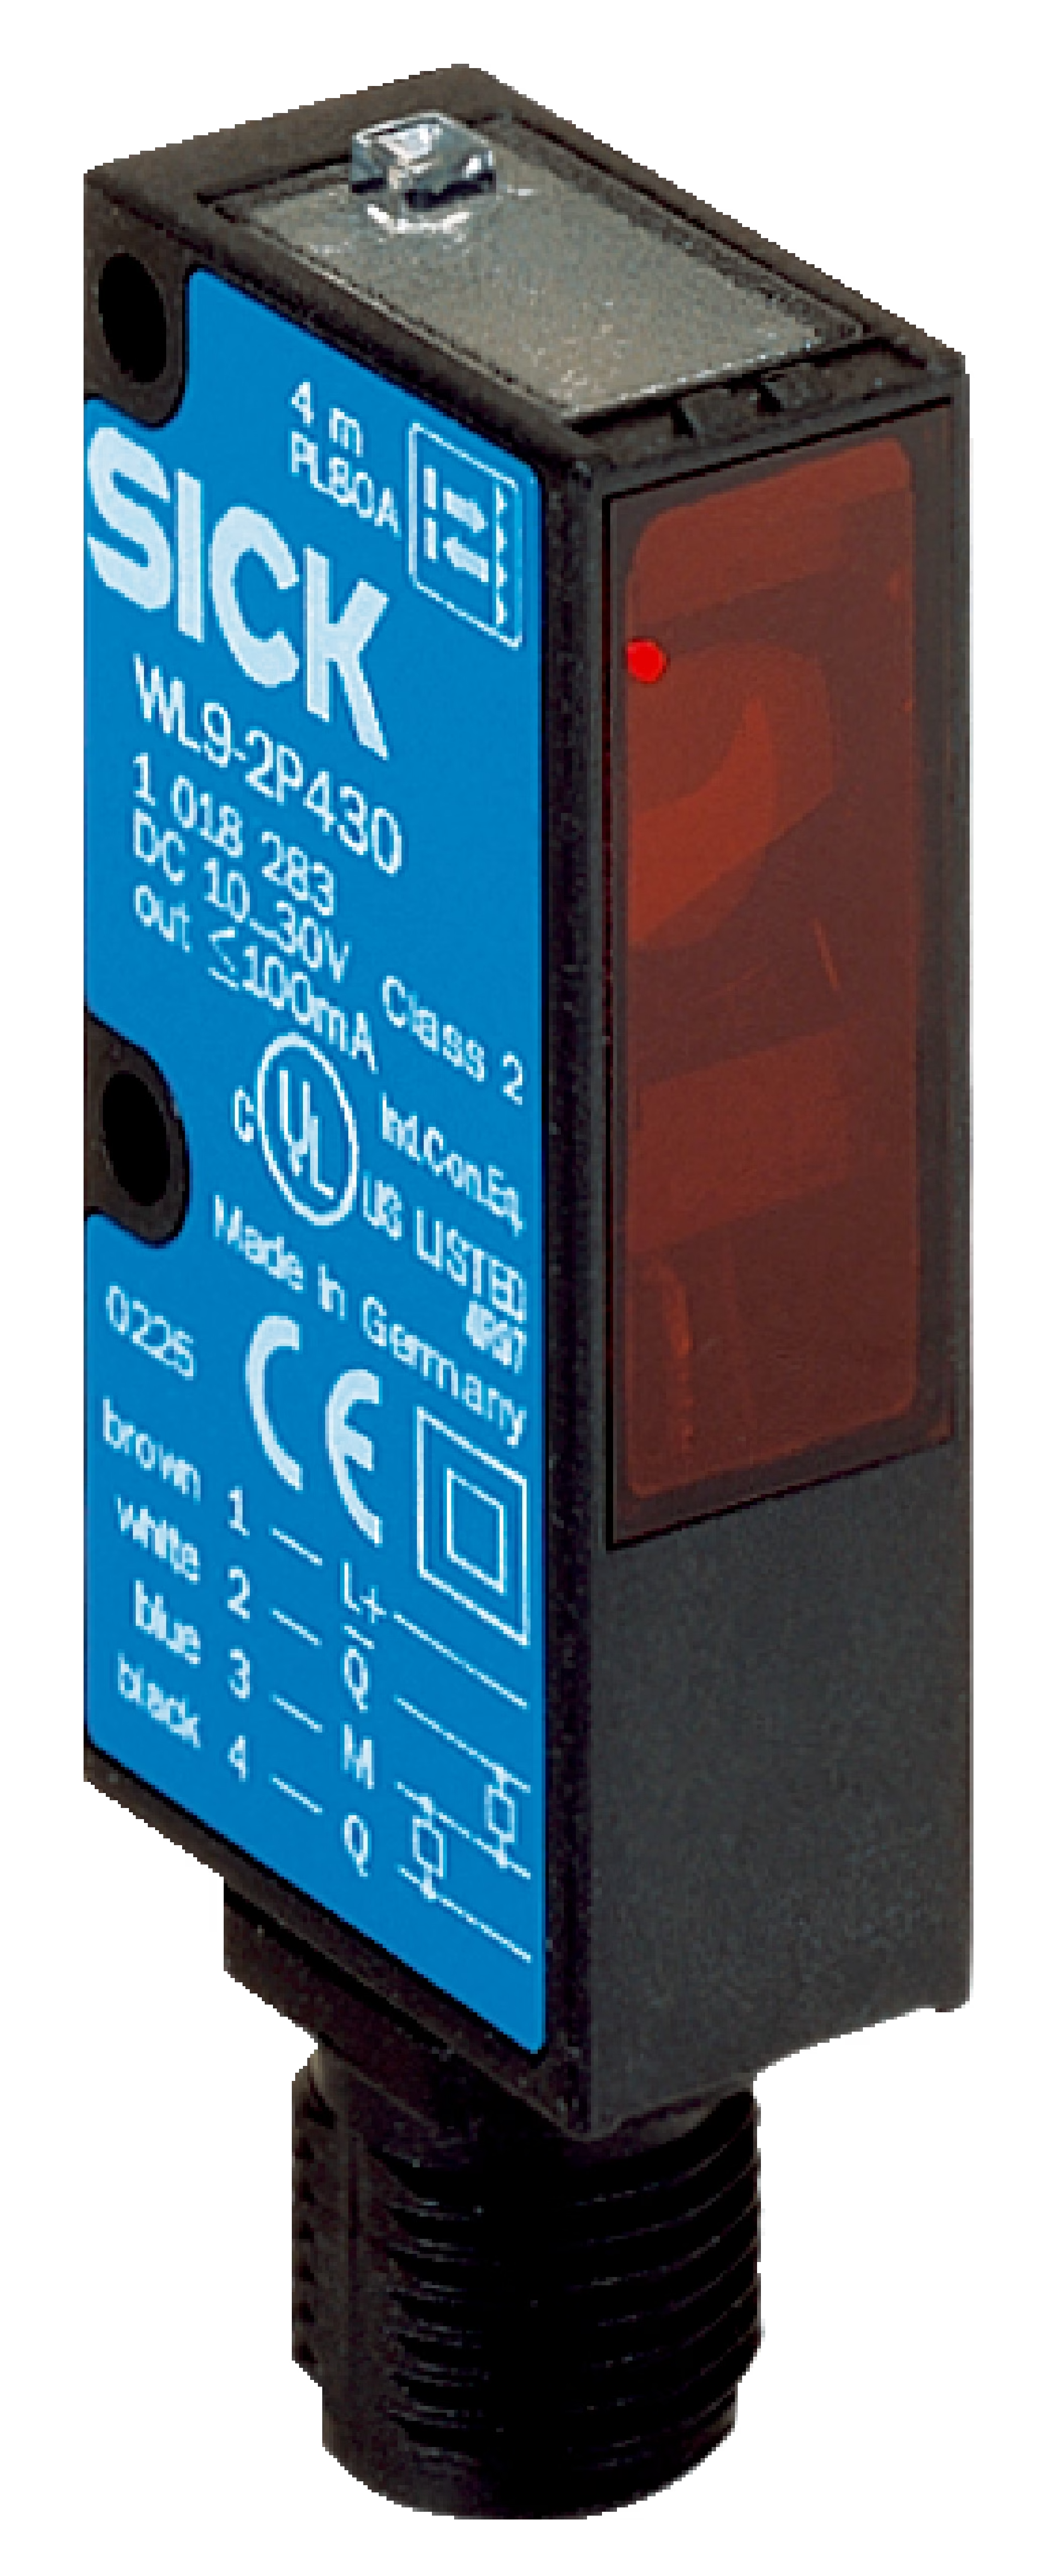
\includegraphics[scale=0.05]{./01_Inhalte/01_Lichtschranke.pdf}	
		\centering
		\caption{Reflexlichtschranke}
		\label{fig:Lichtschranke}
	\end{figure}
\end{minipage}	
\\ \\
Ist diese nicht ausgelöst, ist der Ausgang mit der positiven Eingangsspannung verbunden. Löst die Lichtschranke aus wird der Ausgang auf Masse gezogen. Da der Spannungsbereich der Reflexlichtschranke nicht mit dem des ESP32 übereinstimmt, muss der Ausgang an den Spannungsbereich des ESP32 angepasst werden. Dies wird durch einen Pegelwandler (Level Shifter) erzielt. Weiters ist zu beachten, dass die maximale Reichweite von 4m nur in Verbindung mit dem Reflektor \textbf{PL80A} (Abbildung \ref{fig:PL80A}) erzielt werden kann. Dieser besitzt über eine Reflexionsfläche mit den Maßen 80mm x 80mm.

\begin{figure}[H]
	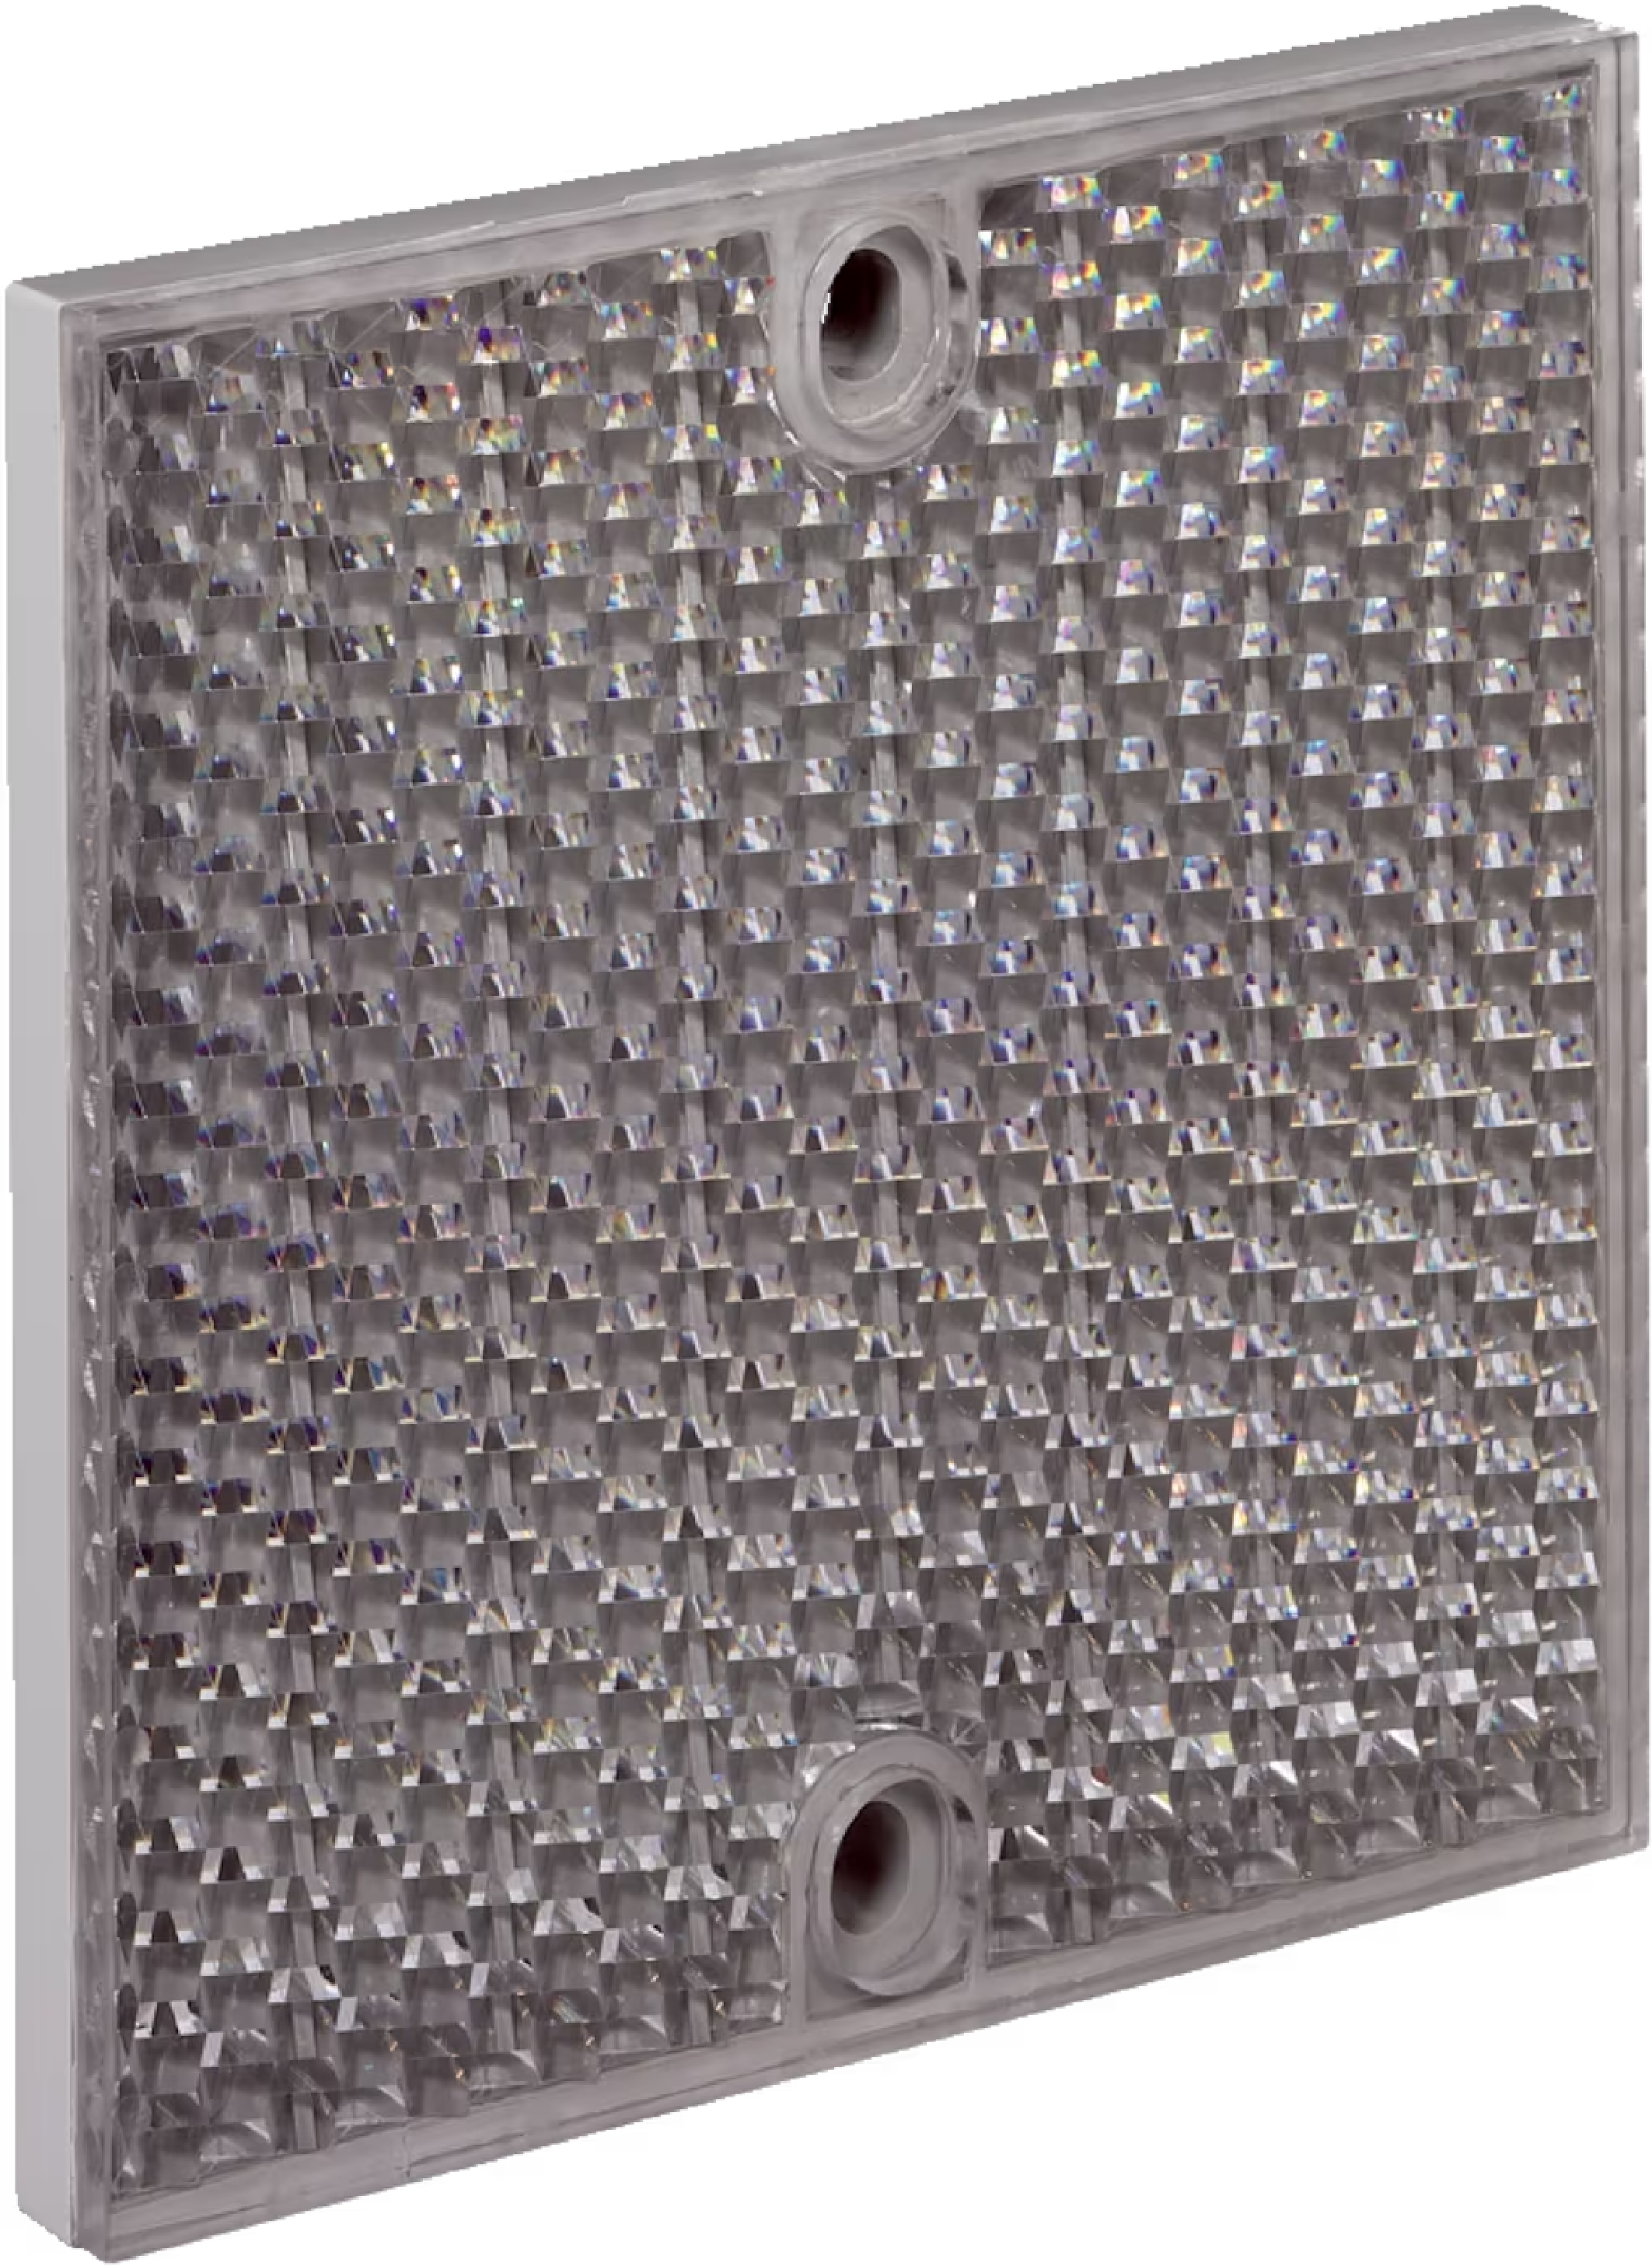
\includegraphics[height=4.6cm]{./01_Inhalte/01a_PL80A.pdf}	
	\centering
	\caption{PL80A-Reflektor}
	\label{fig:PL80A}
\end{figure}


\subsubsection{\ac{µC}}
Als \textbf{\ac{µC}} wird hier der \textbf{ESP32-S2-LCD} der Firma Waveshare verwendet. Standardmäßig ist bereits ein Display verbaut, das später dazu verwendet wird, die Zeitstempel der letzten Auslösung der Lichtschranke anzuzeigen.

\begin{minipage}{0.6\textwidth}
	\begin{itemize}
		\item Xtensa single-core 32-bit LX7 Mikroprozessor
		\item 2.4 GHz WiFi Keramik-Antenne
		\item 0.96-Zoll LCD Display
	\end{itemize}
\end{minipage}%
\begin{minipage}{0.4\textwidth}		
	\begin{figure}[H]
		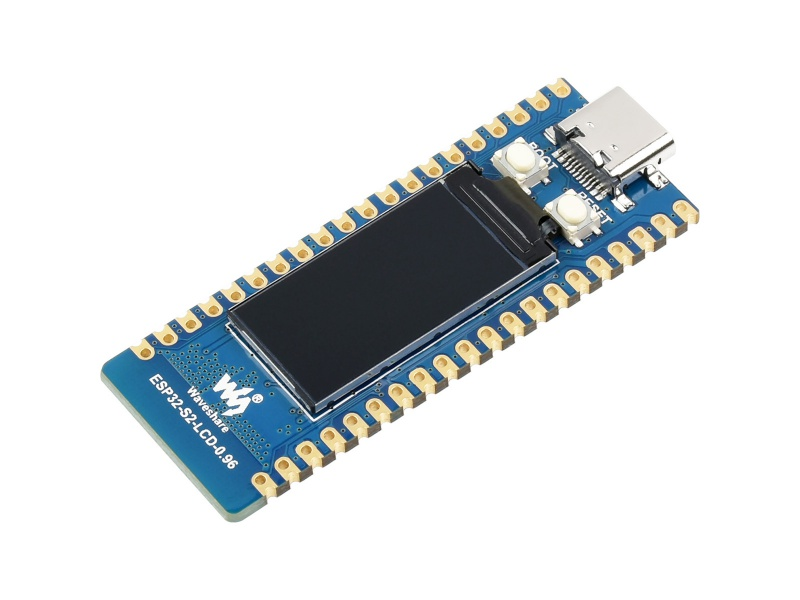
\includegraphics[scale=0.2]{./01_Inhalte/02_ESP32-S2-LCD.jpg}	
		\centering
		\caption{ESP32-S2-LCD}
		\label{fig:ESP32-S2-LCD}
	\end{figure}
\end{minipage}	

\begin{figure}[H]
	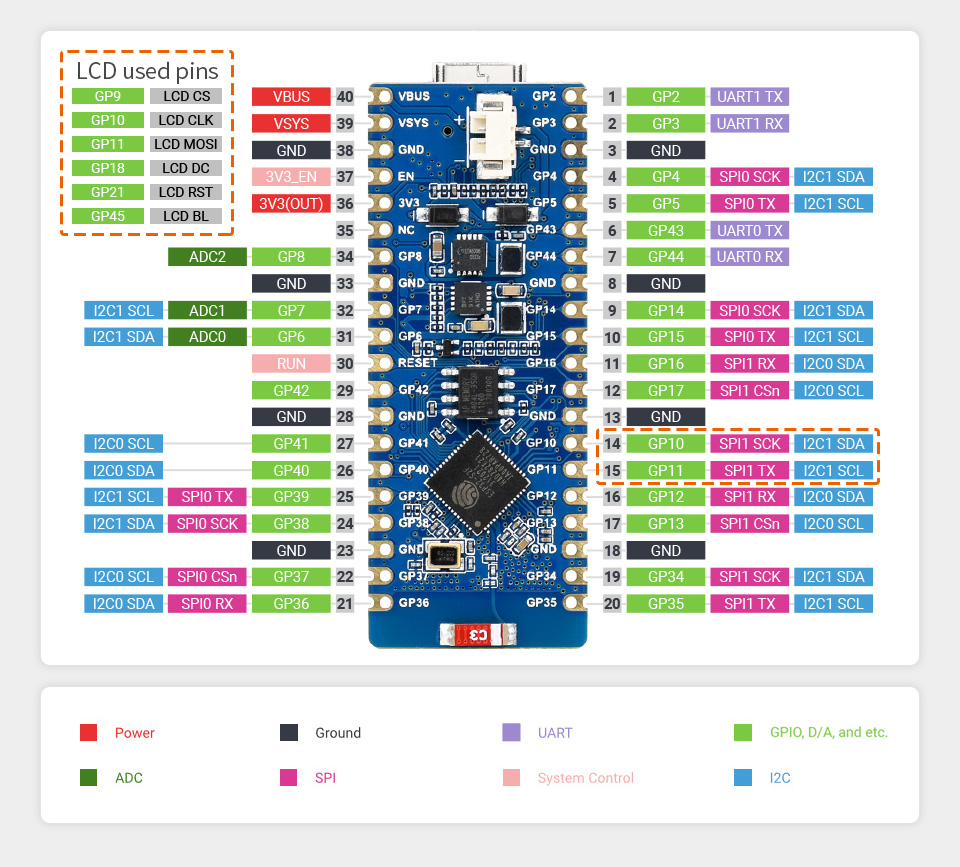
\includegraphics[width=\textwidth]{./01_Inhalte/02a_ESP32-S2-LCD_Pinout.jpg}	
	\centering
	\caption{ESP32-S2-LCD Pinout}
	\label{fig:ESP32-S2-LCD_Pinout}
\end{figure}



\subsubsection{GPS-Modul}
Zur Synchronisation der \textbf{\ac{RTC}} der \acl{µC} wird das GPS Modul \textbf{U-Blox Neo-6MV2} verwendet. Hierdurch wird gewährleistet, dass alle ESP32 exakt dieselbe Zeit bekommen.

\begin{minipage}{0.65\textwidth}
	\begin{itemize}
		\item Versorgungsspannung: 3V DC - 5V DC
		\item Maximaler E / A-Logikpegel: 3.6V
		\item Stromverbrauch: 40mA
		\item Kommunikationsinterface: UART TTL, 9600bps
		\item Zeitgenauigkeit: 1µs
		\item Betriebstemperatur: -40°C - +80°C
	\end{itemize}
\end{minipage}%
\begin{minipage}{0.35\textwidth}		
	\begin{figure}[H]
		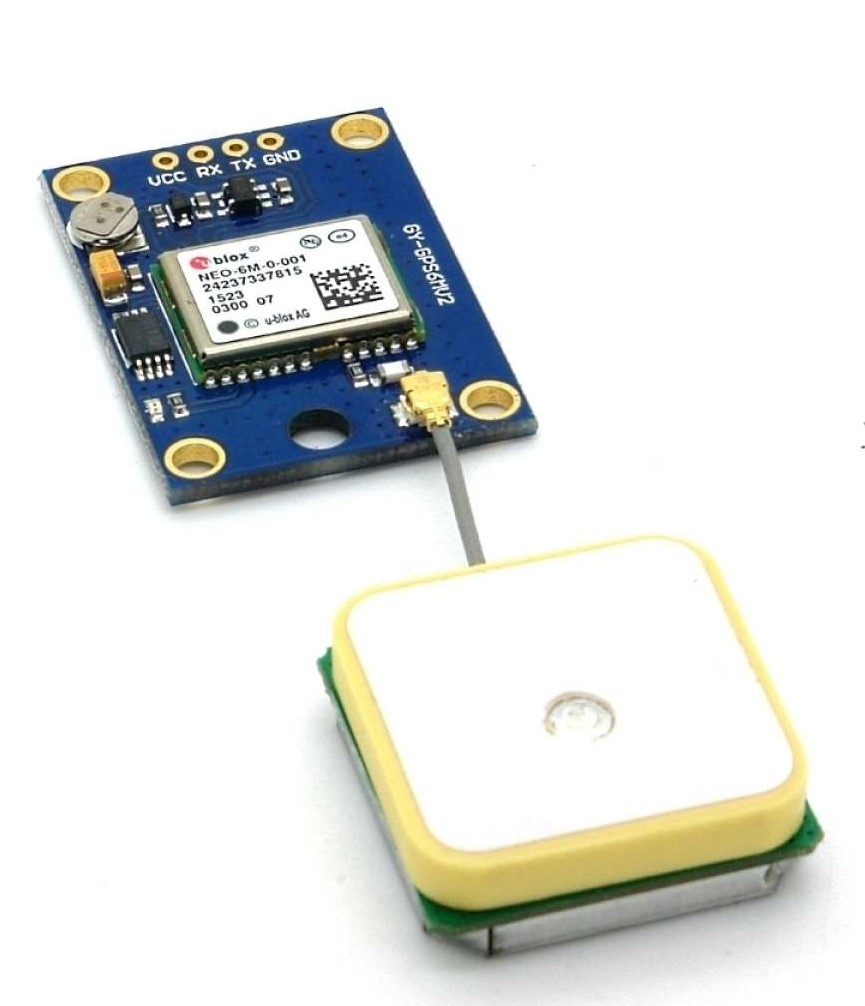
\includegraphics[scale=0.2]{./01_Inhalte/03_GPS-Modul.jpg}	
		\centering
		\caption{U-Box Neo-6M}
		\label{fig:GPS-Modul}
	\end{figure}
\end{minipage}	



\subsubsection{Stromversorgung}
Als Stromversorgung für die Station wird ein handelsüblicher Makita Akku verwendet.

\begin{minipage}{0.6\textwidth}
	\begin{itemize}
		\item Nennspannung: 18V
		\item Entladeschlussspannung: 15V
		\item Ladespannung: 21V 
		\item Kapazität: 108Wh
		\item Akkutyp: Li-ion
	\end{itemize}
\end{minipage}%
\begin{minipage}{0.4\textwidth}		
	\begin{figure}[H]
		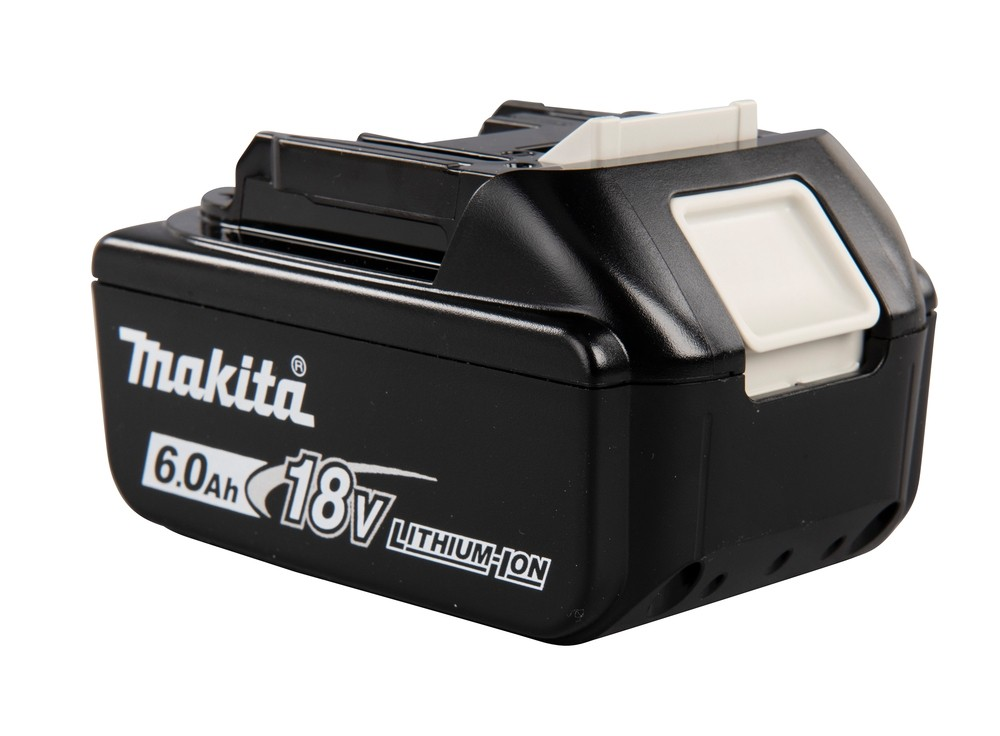
\includegraphics[scale=0.2]{./01_Inhalte/04_Makita-Akku.jpg}	
		\centering
		\caption{Makita-Akku}
		\label{fig:Makita-Akku}
	\end{figure}
\end{minipage}	

\subsubsection{DC-DC Wandler}
Für die Versorgung des ESP32-S2 wird eine Spannung von rund 5V benötigt. Diese wird durch den Buck-Schaltregler \textbf{OKI-78SR-5/1.5-W36-C} der Firma Murata PS bereitgestellt.


\begin{minipage}{0.45\textwidth}
	\begin{itemize}
		\item Eingangspannung: 7-36V DC
		\item Ausgangsspannung: 5V
		\item Maximaler Ausgangsstrom: 1,5A
	\end{itemize}
\end{minipage}%
\begin{minipage}{0.55\textwidth}		
	\begin{figure}[H]
		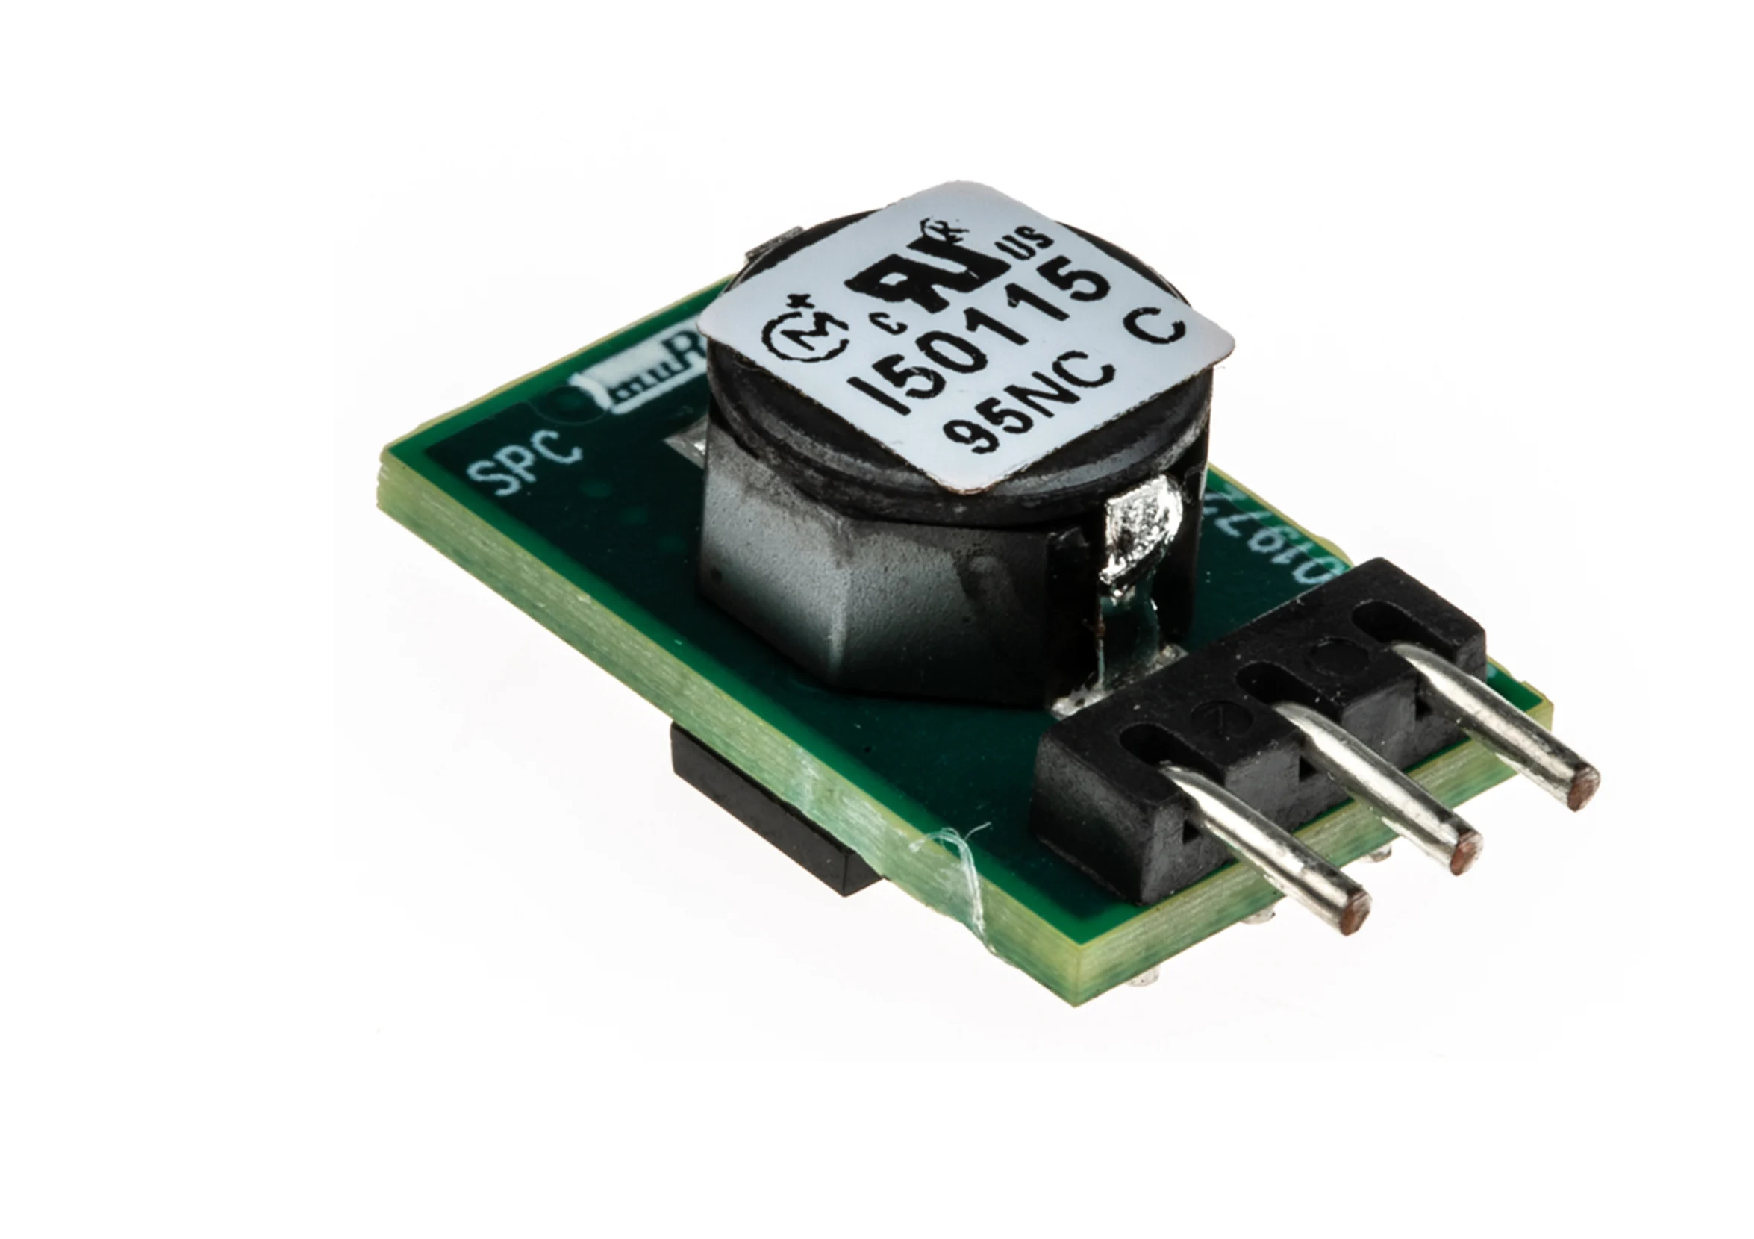
\includegraphics[scale=0.2]{./01_Inhalte/05_DC-DC.pdf}	
		\centering
		\caption{Murata PS OKI-78SR-5/1.5-W36-C}
		\label{fig:DC-DC}
	\end{figure}
\end{minipage}	


\subsubsection{Schaltplan}
Die vorher genannten Bauelemente werden wie in Abbildung \ref{fig:Lichtschranke-Schaltplan} dargestellt verschalten. Hinzu kommt noch der in Kapitel \ref{sec:Lichtschranke} genannte Pegelwandler mittels eines NPN-Transistors. Löst die Lichtschranke aus liegt an ihrem Ausgang (Q) eine Pegel von 0V an. Durch das Level Shifting liegt dadurch am GPIO15-Pin des ESP32 ein Spannungspegel von 3,3V an.

\begin{figure}[H]
	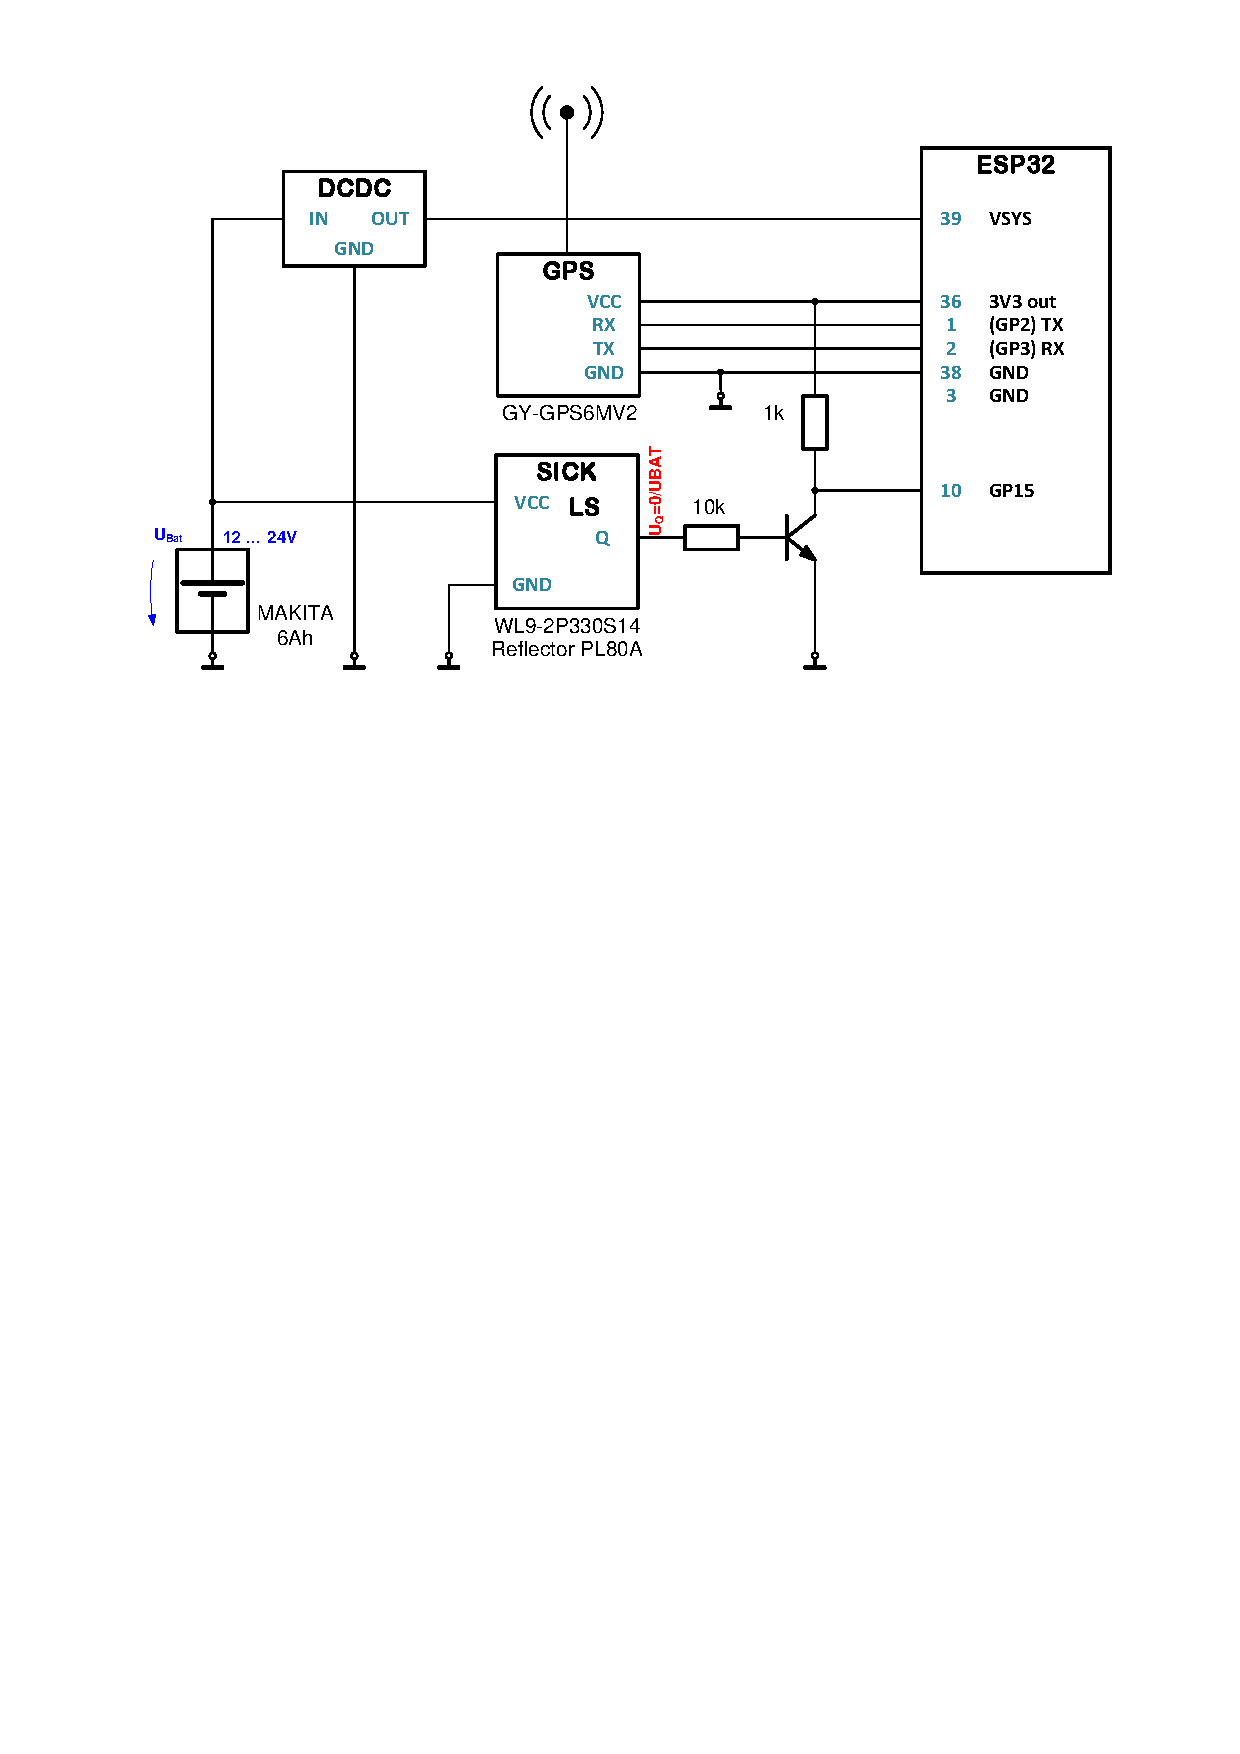
\includegraphics[width=\textwidth]{./01_Inhalte/06_Lichtschranke-Schaltplan.pdf}	
	\centering
	\caption{Lichtschranke-Schaltplan}
	\label{fig:Lichtschranke-Schaltplan}
\end{figure}


\subsection{MQTT}
Alle Zeitstempel werden über das WLAN mittels \textbf{MQTT} übertragen. Bei jedem Verbindungsaufbau mit dem MQTT-Broker wird im Topic \textbf{''clients''} der Name der Station übertragen \textbf{(''ESP32-'' + Mac-Adresse)}. Alle erfassten Zeitstempel der Lichtschranken-Stationen werden im Topic \textbf{''esp32/timestamps''} veröffentlicht. 

\subsection{Zeit-Synchronisierung}
Bei jedem Neustart oder erstmaligen Starten erfolgt eine Synchronisierung der Echtzeituhr (\ac{RTC}) mit dem GPS-Modul. Dies gewährleistet, dass jede Station über genau dieselbe Zeit verfügt.

\subsection{Lichtschranke}
Löst die Lichtschranke aus wird der \textbf{GPIO15-Pin} auf High (3,3V) gezogen. Softwaretechnisch löst dies eine \textbf{Interrupt-Routine } aus, in welcher die Zeit aus der \ac{RTC} auf Mikrosekunden genau ausgelesen wird. Im Loop wird dann dieser Zeitstempel weiterverarbeitet und am Display angezeigt bzw. an den MQTT-Broker gesendet.


\subsection{Implementierungsschritte}
Um das Programm auf den Arduino zu laden empfehle ich \textbf{Platformio} in VS-Code zu verwenden. In Platformio muss man den Projektordner ''\textbf{03\_LichtschrankenStation}'' öffnen. Zudem müssen einige Änderungen im Programmcode des ESP32 vorgenommen werden, damit der Code funktioniert. Grundsätzlich muss der Server sich im gleichem lokalem Netzwerk befinden wie die Lichtschranken-Stationen, somit muss die \textbf{SSID} \& das \textbf{Passwort} angepasst werden. Zudem muss man noch die \textbf{IP-Adresse} des Servers eintragen und die Benutzerdaten anpassen, falls diese geändert wurden. Diese Anpassungen müssen in der Datei \textbf{main.cpp}, die sich im Verzeichnis \textbf{/03\_LichtschrankenStation/src/} befindet, vorgenommen werden, um eine korrekte Verbindung zum Server zu gewährleisten.

\begin{lstlisting}[language=myCpp]
	// WiFi credentials
	const char* wifi_ssid = "SSID";          
	const char* wifi_password = "PASSWORD";  
	
	// MQTT server configuration
	const char* mqtt_server = "SERVER-IP";  
	const char* mqtt_user = "mqttclient";    
	const char* mqtt_password = "Kennwort1";  
\end{lstlisting}

Nach Durchführung dieser Modifikationen kann der Code kompiliert und auf den ESP32 geladen werden. Bevor man den Code auf den ESP32 lädt, musst man sicherstellen, dass das Gerät im Boot-Modus ist. Folgende Schritte müssen hierfür durchgeführt werden:

\begin{itemize}
	\item Schließe den ESP32 an den Computer an.
	\item Drücke und halte die BOOT-Taste, und drücke dann die RESET-Taste.
	\item Lasse zuerst die RESET-Taste los und dann die BOOT-Taste.
\end{itemize}

Da wir manuell den Boot-Modus aktiviert haben, wird bei der Übertragung eine Fehlermeldung auftauchen, die jedoch ignoriert werden kann. Nach Übertragung des Codes muss der ESP32 manuell neugestartet werden, indem man die \textbf{RESET-Taste} drückt.